\chapter{Background}\label{chap:Background}

\begin{Listing}[t]
\centering
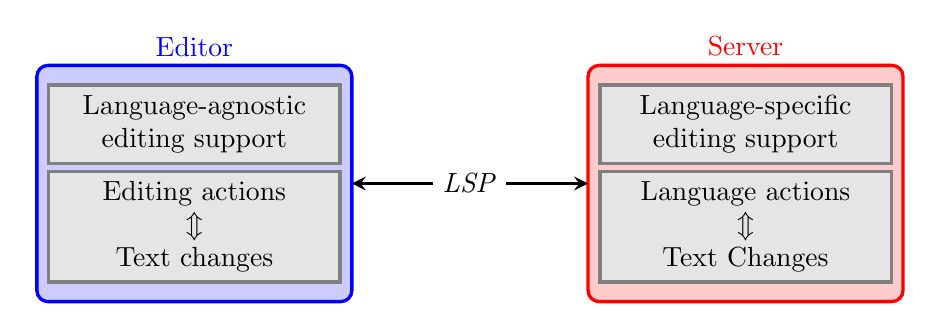
\begin{tikzpicture}
\draw[blue, very thick, rounded corners, fill=blue!20, anchor=north]
        (0,0) rectangle (4,3)
        node[anchor=north, align=center] at (2,3.5) {Editor};
\draw[gray, very thick, fill=gray!20]
        (0.15, 1.75) rectangle (3.85,2.75)
        node[black, text width=4cm, pos=.5, align=center] {Language-agnostic \linebreak editing support};
\draw[gray, very thick, fill=gray!20]
        (0.15, 0.25) rectangle (3.85,1.65)
        node[black, text width=4cm, pos=.5, align=center] {Editing actions \linebreak $\Updownarrow$ \linebreak  Text changes};

\draw[red, very thick, rounded corners, fill=red!20, anchor=north]
        (7,0) rectangle (11,3)
        node[anchor=north, align=center] at (9,3.5) {Server};
\draw[gray, very thick, fill=gray!20]
        (7.15, 1.75) rectangle (10.85,2.75)
        node[black, text width=4cm, pos=.5, align=center] {Language-specific \linebreak editing support};
\draw[gray, very thick, fill=gray!20]
        (7.15, 0.25) rectangle (10.85,1.65)
        node[black, text width=4cm, pos=.5, align=center] {Language actions \linebreak $\Updownarrow$ \linebreak Text Changes};

\draw[<->, very thick, >=stealth] (4,1.5) -- (7,1.5)
        node[midway,fill=white] {\emph{LSP}};
\end{tikzpicture}
\caption{LSP approach to language support. Borrowed from \cite{Rodriguez-Echeverria18a}}
\label{lst:lsp}
\end{Listing}

In this chapter, we provide an overview of the concepts and technologies that are relevant to the work presented in this thesis. We start by introducing the concept of language servers and the Language Server Protocol (LSP) in Section~\ref{sec:LanguageServerProtocol}. We then discuss language workbenches in Section~\ref{sec:LanguageWorkbenches}, type systems in Section~\ref{sec:TypeSystems}, and software and language product lines in Section~\ref{sec:SoftwareProductLines}.

The goal of this chapter is to provide the reader with the necessary background knowledge to understand the work presented in the following chapters. We assume that the reader has a basic understanding of programming languages and software development.

\section{Language Server Protocol}\label{sec:LanguageServerProtocol}
% Introduction to the Language Server Protocol
The Language Server Protocol\footnote{\url{https://microsoft.github.io/language-server-protocol}} (LSP) is a protocol that allows for the communication between a language server and an editor or an IDE. The LSP is used to decuple the a language-agnotic editor or integrated development environment (IDE) from the language-specific features of a language server (see Listing~\ref{lst:lsp}). This allows for the development of language servers that can be used with multiple editors or IDEs. The LSP is based on the stateless JSON-RPC protocol and defines a set of messages that are used to communicate between the language server and the editor or IDE.

Usually, the LSP Clients are developed as plugins for popular editors or IDEs decresing the effort to support a new language in a given editor. The LSP Clients are responsible for sending requests to the language server and processing the responses. The language server is responsible for providing language-specific features. The LSP defines a set of messages that are used to communicate between the language server and the editor or IDE. These messages include requests for code completion, code navigation, and code analysis, as well as notifications for changes to the document, diagnostics, and progress reports.

Language servers are \textit{de facto} standard for providing language-specific features in editors and IDEs. The LSP is supported by a wide range of editors and IDEs, including Noevim\footnote{\url{https://neovim.io/doc/user/lsp.html}}, Visual Studio Code\footnote{\url{https://code.visualstudio.com/api/language-extensions/language-server-extension-guide}}, Eclipse\footnote{\url{https://www.eclipse.org/community/eclipse_newsletter/2017/may/article1.php}}, and IntelliJ IDEA\footnote{\url{https://plugins.jetbrains.com/docs/intellij/language-server-protocol.html}}. There are several language servers available for popular programming languages, including Rust, TypeScript, Python, and Java and most of them are open-source\footnote{\url{https://microsoft.github.io/language-server-protocol/implementors/servers}}.

The LSP is initiated by Microsoft and is now an open standard that is maintained by the Language Server Protocol Working Group. It was designed for the use with the Visual Studio Code editor, but it has since been adopted by other editors and IDEs. The LSP is under open-source license and is available on GitHub\footnote{\url{https://github.com/microsoft/language-server-protocol}}.

\subsection{JSON-RPC}\label{subsec:JSONRPC}
The LSP uses JSON-RPC to communicate between a language server and an editor. JSON-RPC (v2)\footnote{\url{https://www.jsonrpc.org/specification}} is a stateless, light-weight remote procedure call (RPC) \cite{Birrell84} protocol that uses JSON as the data format.

RPC is a protocol that allows a client to call a procedure on a remote server. The client sends a request to the server, and the server sends a response back to the client. The JSON-RPC protocol defines a set of messages that are used to communicate between the client and the server. These messages include requests, responses, and notifications. The JSON-RPC protocol is designed to be simple and easy to implement, making it well-suited for use in web applications and other distributed systems.

JSON-RPC is a JSON based implementation of the RPC protocol. It defines a set of rules for encoding and decoding JSON data, as well as a set of rules for \textit{Request}, \textit{Notification}, and \textit{Response} messages. The messages are sent over a transport layer, such as HTTP or WebSockets. The JSON-RPC protocol is designed to be simple and easy to implement, making it well-suited for use in web applications and other distributed systems.

All messages refer to a \textit{method} that is a string containing the name of the method to be called. The \textit{params} field is an array or object containing the parameters to be passed to the method. Typically, messages are synchronous, meaning that the client waits for a response from the server before continuing. The \textit{id} field is a unique identifier for the message, which is used to match requests with responses. However, the JSON-RPC protocol also supports asynchronous messages, known as notifications, which do not require a response from the server. This is implemented by setting the \textit{id} field to \textit{null}, in which case the server does not send a response back to the client.

The JSON-RPC specification includes the ability for clients to batch multiple requests or notifications by sending them as a list. The server is expected to respond with a corresponding list of results for each request. Additionally, the server has the flexibility to process these requests concurrently.

\section{Language Workbenches}\label{sec:LanguageWorkbenches}

\section{Type Systems}\label{sec:TypeSystems}

\section{Software and Language Product Lines}\label{sec:SoftwareProductLines}
